%%%%%%%%%%%%%%%%%%%%%%%%%%%%%%%%%%%%%%%%%%%%%%%%%%%%%%%%%%%%%%%%%%%%%%%%

%%% LaTeX Template for AAMAS-2025 (based on sample-sigconf.tex)
%%% Prepared by the AAMAS-2025 Program Chairs based on the version from AAMAS-2025. 

%%%%%%%%%%%%%%%%%%%%%%%%%%%%%%%%%%%%%%%%%%%%%%%%%%%%%%%%%%%%%%%%%%%%%%%%

%%% Start your document with the \documentclass command.


%%% == IMPORTANT ==
%%% Use the first variant below for the final paper (including auithor information).
%%% Use the second variant below to anonymize your submission (no authoir information shown).
%%% For further information on anonymity and double-blind reviewing, 
%%% please consult the call for paper information
%%% https://aamas2025.org/index.php/conference/calls/submission-instructions-main-technical-track/

%%%% For anonymized submission, use this
\documentclass[sigconf,nonacm]{aamas} 

%%%% For camera-ready, use this
%\documentclass[sigconf]{aamas} 


%%% Load required packages here (note that many are included already).

\usepackage{balance} % for balancing columns on the final page
\usepackage{tikz}
\usepackage{graphicx}
\usepackage{float}
\usepackage{dblfloatfix}
\usepackage{placeins}
\usepackage{afterpage}
\usepackage{algorithm}
\usepackage[noend]{algpseudocode}
\usepackage{amsmath}
%\usepackage{amssymb}
\usepackage{amsthm}

%\theoremstyle{plain}
\newtheorem{theorem}{Theorem}[section]
\newtheorem{observation}[theorem]{Observation}

%%%%%%%%%%%%%%%%%%%%%%%%%%%%%%%%%%%%%%%%%%%%%%%%%%%%%%%%%%%%%%%%%%%%%%%%

%%% AAMAS-2025 copyright block (do not change!)

\setcopyright{ifaamas}
\acmConference[AAMAS '25]{Proc.\@ of the 24th International Conference
on Autonomous Agents and Multiagent Systems (AAMAS 2025)}{May 19 -- 23, 2025}
{Detroit, Michigan, USA}{A.~El~Fallah~Seghrouchni, Y.~Vorobeychik, S.~Das, A.~Nowe (eds.)}
\copyrightyear{2025}
\acmYear{2025}
\acmDOI{}
\acmPrice{}
\acmISBN{}


%%%%%%%%%%%%%%%%%%%%%%%%%%%%%%%%%%%%%%%%%%%%%%%%%%%%%%%%%%%%%%%%%%%%%%%%

%%% == IMPORTANT ==
%%% Use this command to specify your EasyChair submission number.
%%% In anonymous mode, it will be printed on the first page.

\acmSubmissionID{<<EasyChair submission id>>}

%%% Use this command to specify the title of your paper.

\title[AAMAS-2025 Formatting Instructions]{Interval Selection with Binary Predictions}

%%% Provide names, affiliations, and email addresses for all authors.

\author{Christodoulos Karavasilis}
\affiliation{
  \institution{University of Toronto}
  \city{Toronto}
  \country{Canada}}
\email{ckar@cs.toronto.edu}


%%% Use this environment to specify a short abstract for your paper.

\begin{abstract}
Following a line of work that takes advantage of vast machine-learned data to enhance online algorithms with (possibly erroneous) information about future inputs, we consider predictions in the context of deterministic algorithms for the problem of selecting a maximum weight independent set of intervals arriving on the real line. We look at two weight functions, unit (constant) weights, and weights proportional to the interval's length. In the classical online model of irrevocable decisions, no algorithm can achieve constant competitiveness (Bachmann et al. \cite{bachmann2013online} for unit, Lipton and Tomkins \cite{lipton1994online} for proportional). In this setting, we show that a simple algorithm that is faithful to the predictions is optimal, and achieves an objective value of at least $OPT-\eta$, with $\eta$ being the total error in the predictions, both for unit, and proportional weights.

When revocable acceptances (a form of \textit{preemption}) are allowed, the optimal deterministic algorithm for unit weights is $2k$-competitive \cite{borodin2023any}, where $k$ is the number of different interval lengths. We give an algorithm with performance $OPT -\eta$ (and therefore $1$-consistent), that is also $(2k+1)$-robust. For proportional weights, Garay et al. \cite{garay1997efficient} give an optimal $(2\phi +1)$-competitive algorithm, where $\phi$ is the golden ratio. We present an algorithm with parameter $\lambda > 1$ that is $\frac{3\lambda}{\lambda -1}$-consistent, and $\frac{4\lambda^2 + 2\lambda}{\lambda -1}$-robust. Although these bounds are not tight, we show that for $\lambda > 3.42$ we achieve consistency better than the optimal online guarantee in \cite{garay1997efficient}, while maintaining bounded robustness.

 We conclude with some experimental results on real-world data that complement our theoretical findings, and show the benefit of prediction algorithms for online interval selection, even in the presence of high error.
\end{abstract}

%%% The code below was generated by the tool at http://dl.acm.org/ccs.cfm.
%%% Please replace this example with code appropriate for your own paper.


%%% Use this command to specify a few keywords describing your work.
%%% Keywords should be separated by commas.

\keywords{online algorithms, predictions, interval selection, scheduling}

%%%%%%%%%%%%%%%%%%%%%%%%%%%%%%%%%%%%%%%%%%%%%%%%%%%%%%%%%%%%%%%%%%%%%%%%

%%% Include any author-defined commands here.
         
\newcommand{\BibTeX}{\rm B\kern-.05em{\sc i\kern-.025em b}\kern-.08em\TeX}

%%%%%%%%%%%%%%%%%%%%%%%%%%%%%%%%%%%%%%%%%%%%%%%%%%%%%%%%%%%%%%%%%%%%%%%%

\begin{document}

%%% The following commands remove the headers in your paper. For final 
%%% papers, these will be inserted during the pagination process.

\pagestyle{fancy}
\fancyhead{}

%%% The next command prints the information defined in the preamble.

\maketitle 

%%%%%%%%%%%%%%%%%%%%%%%%%%%%%%%%%%%%%%%%%%%%%%%%%%%%%%%%%%%%%%%%%%%%%%%%

\section{Introduction}
\section{Introduction}


\begin{figure}[t]
\centering
\includegraphics[width=0.6\columnwidth]{figures/evaluation_desiderata_V5.pdf}
\vspace{-0.5cm}
\caption{\systemName is a platform for conducting realistic evaluations of code LLMs, collecting human preferences of coding models with real users, real tasks, and in realistic environments, aimed at addressing the limitations of existing evaluations.
}
\label{fig:motivation}
\end{figure}

\begin{figure*}[t]
\centering
\includegraphics[width=\textwidth]{figures/system_design_v2.png}
\caption{We introduce \systemName, a VSCode extension to collect human preferences of code directly in a developer's IDE. \systemName enables developers to use code completions from various models. The system comprises a) the interface in the user's IDE which presents paired completions to users (left), b) a sampling strategy that picks model pairs to reduce latency (right, top), and c) a prompting scheme that allows diverse LLMs to perform code completions with high fidelity.
Users can select between the top completion (green box) using \texttt{tab} or the bottom completion (blue box) using \texttt{shift+tab}.}
\label{fig:overview}
\end{figure*}

As model capabilities improve, large language models (LLMs) are increasingly integrated into user environments and workflows.
For example, software developers code with AI in integrated developer environments (IDEs)~\citep{peng2023impact}, doctors rely on notes generated through ambient listening~\citep{oberst2024science}, and lawyers consider case evidence identified by electronic discovery systems~\citep{yang2024beyond}.
Increasing deployment of models in productivity tools demands evaluation that more closely reflects real-world circumstances~\citep{hutchinson2022evaluation, saxon2024benchmarks, kapoor2024ai}.
While newer benchmarks and live platforms incorporate human feedback to capture real-world usage, they almost exclusively focus on evaluating LLMs in chat conversations~\citep{zheng2023judging,dubois2023alpacafarm,chiang2024chatbot, kirk2024the}.
Model evaluation must move beyond chat-based interactions and into specialized user environments.



 

In this work, we focus on evaluating LLM-based coding assistants. 
Despite the popularity of these tools---millions of developers use Github Copilot~\citep{Copilot}---existing
evaluations of the coding capabilities of new models exhibit multiple limitations (Figure~\ref{fig:motivation}, bottom).
Traditional ML benchmarks evaluate LLM capabilities by measuring how well a model can complete static, interview-style coding tasks~\citep{chen2021evaluating,austin2021program,jain2024livecodebench, white2024livebench} and lack \emph{real users}. 
User studies recruit real users to evaluate the effectiveness of LLMs as coding assistants, but are often limited to simple programming tasks as opposed to \emph{real tasks}~\citep{vaithilingam2022expectation,ross2023programmer, mozannar2024realhumaneval}.
Recent efforts to collect human feedback such as Chatbot Arena~\citep{chiang2024chatbot} are still removed from a \emph{realistic environment}, resulting in users and data that deviate from typical software development processes.
We introduce \systemName to address these limitations (Figure~\ref{fig:motivation}, top), and we describe our three main contributions below.


\textbf{We deploy \systemName in-the-wild to collect human preferences on code.} 
\systemName is a Visual Studio Code extension, collecting preferences directly in a developer's IDE within their actual workflow (Figure~\ref{fig:overview}).
\systemName provides developers with code completions, akin to the type of support provided by Github Copilot~\citep{Copilot}. 
Over the past 3 months, \systemName has served over~\completions suggestions from 10 state-of-the-art LLMs, 
gathering \sampleCount~votes from \userCount~users.
To collect user preferences,
\systemName presents a novel interface that shows users paired code completions from two different LLMs, which are determined based on a sampling strategy that aims to 
mitigate latency while preserving coverage across model comparisons.
Additionally, we devise a prompting scheme that allows a diverse set of models to perform code completions with high fidelity.
See Section~\ref{sec:system} and Section~\ref{sec:deployment} for details about system design and deployment respectively.



\textbf{We construct a leaderboard of user preferences and find notable differences from existing static benchmarks and human preference leaderboards.}
In general, we observe that smaller models seem to overperform in static benchmarks compared to our leaderboard, while performance among larger models is mixed (Section~\ref{sec:leaderboard_calculation}).
We attribute these differences to the fact that \systemName is exposed to users and tasks that differ drastically from code evaluations in the past. 
Our data spans 103 programming languages and 24 natural languages as well as a variety of real-world applications and code structures, while static benchmarks tend to focus on a specific programming and natural language and task (e.g. coding competition problems).
Additionally, while all of \systemName interactions contain code contexts and the majority involve infilling tasks, a much smaller fraction of Chatbot Arena's coding tasks contain code context, with infilling tasks appearing even more rarely. 
We analyze our data in depth in Section~\ref{subsec:comparison}.



\textbf{We derive new insights into user preferences of code by analyzing \systemName's diverse and distinct data distribution.}
We compare user preferences across different stratifications of input data (e.g., common versus rare languages) and observe which affect observed preferences most (Section~\ref{sec:analysis}).
For example, while user preferences stay relatively consistent across various programming languages, they differ drastically between different task categories (e.g. frontend/backend versus algorithm design).
We also observe variations in user preference due to different features related to code structure 
(e.g., context length and completion patterns).
We open-source \systemName and release a curated subset of code contexts.
Altogether, our results highlight the necessity of model evaluation in realistic and domain-specific settings.






%%%%%%%%%%%%%%%%%%%%%%%%%%%%%%%%%%%%%%%%%%%%%%%%%%%%%%%%%%%%%%%%%%%%%%%%

\section{Problem Setting, Definitions and Discussion} \label{section:prelim}
\section{Preliminaries}
\label{sec:prelim}
\label{sec:term}
We define the key terminologies used, primarily focusing on the hidden states (or activations) during the forward pass. 

\paragraph{Components in an attention layer.} We denote $\Res$ as the residual stream. We denote $\Val$ as Value (states), $\Qry$ as Query (states), and $\Key$ as Key (states) in one attention head. The \attlogit~represents the value before the softmax operation and can be understood as the inner product between  $\Qry$  and  $\Key$. We use \Attn~to denote the attention weights of applying the SoftMax function to \attlogit, and ``attention map'' to describe the visualization of the heat map of the attention weights. When referring to the \attlogit~from ``$\tokenB$'' to  ``$\tokenA$'', we indicate the inner product  $\langle\Qry(\tokenB), \Key(\tokenA)\rangle$, specifically the entry in the ``$\tokenB$'' row and ``$\tokenA$'' column of the attention map.

\paragraph{Logit lens.} We use the method of ``Logit Lens'' to interpret the hidden states and value states \citep{belrose2023eliciting}. We use \logit~to denote pre-SoftMax values of the next-token prediction for LLMs. Denote \readout~as the linear operator after the last layer of transformers that maps the hidden states to the \logit. 
The logit lens is defined as applying the readout matrix to residual or value states in middle layers. Through the logit lens, the transformed hidden states can be interpreted as their direct effect on the logits for next-token prediction. 

\paragraph{Terminologies in two-hop reasoning.} We refer to an input like “\Src$\to$\brga, \brgb$\to$\Ed” as a two-hop reasoning chain, or simply a chain. The source entity $\Src$ serves as the starting point or origin of the reasoning. The end entity $\Ed$ represents the endpoint or destination of the reasoning chain. The bridge entity $\Brg$ connects the source and end entities within the reasoning chain. We distinguish between two occurrences of $\Brg$: the bridge in the first premise is called $\brga$, while the bridge in the second premise that connects to $\Ed$ is called $\brgc$. Additionally, for any premise ``$\tokenA \to \tokenB$'', we define $\tokenA$ as the parent node and $\tokenB$ as the child node. Furthermore, if at the end of the sequence, the query token is ``$\tokenA$'', we define the chain ``$\tokenA \to \tokenB$, $\tokenB \to \tokenC$'' as the Target Chain, while all other chains present in the context are referred to as distraction chains. Figure~\ref{fig:data_illustration} provides an illustration of the terminologies.

\paragraph{Input format.}
Motivated by two-hop reasoning in real contexts, we consider input in the format $\bos, \text{context information}, \query, \answer$. A transformer model is trained to predict the correct $\answer$ given the query $\query$ and the context information. The context compromises of $K=5$ disjoint two-hop chains, each appearing once and containing two premises. Within the same chain, the relative order of two premises is fixed so that \Src$\to$\brga~always precedes \brgb$\to$\Ed. The orders of chains are randomly generated, and chains may interleave with each other. The labels for the entities are re-shuffled for every sequence, choosing from a vocabulary size $V=30$. Given the $\bos$ token, $K=5$ two-hop chains, \query, and the \answer~tokens, the total context length is $N=23$. Figure~\ref{fig:data_illustration} also illustrates the data format. 

\paragraph{Model structure and training.} We pre-train a three-layer transformer with a single head per layer. Unless otherwise specified, the model is trained using Adam for $10,000$ steps, achieving near-optimal prediction accuracy. Details are relegated to Appendix~\ref{app:sec_add_training_detail}.


% \RZ{Do we use source entity, target entity, and mediator entity? Or do we use original token, bridge token, end token?}





% \paragraph{Basic notations.} We use ... We use $\ve_i$ to denote one-hot vectors of which only the $i$-th entry equals one, and all other entries are zero. The dimension of $\ve_i$ are usually omitted and can be inferred from contexts. We use $\indicator\{\cdot\}$ to denote the indicator function.

% Let $V > 0$ be a fixed positive integer, and let $\vocab = [V] \defeq \{1, 2, \ldots, V\}$ be the vocabulary. A token $v \in \vocab$ is an integer in $[V]$ and the input studied in this paper is a sequence of tokens $s_{1:T} \defeq (s_1, s_2, \ldots, s_T) \in \vocab^T$ of length $T$. For any set $\mathcal{S}$, we use $\Delta(\mathcal{S})$ to denote the set of distributions over $\mathcal{S}$.

% % to a sequence of vectors $z_1, z_2, \ldots, z_T \in \real^{\dout}$ of dimension $\dout$ and length $T$.

% Let $\mU = [\vu_1, \vu_2, \ldots, \vu_V]^\transpose \in \real^{V\times d}$ denote the token embedding matrix, where the $i$-th row $\vu_i \in \real^d$ represents the $d$-dimensional embedding of token $i \in [V]$. Similarly, let $\mP = [\vp_1, \vp_2, \ldots, \vp_T]^\transpose \in \real^{T\times d}$ denote the positional embedding matrix, where the $i$-th row $\vp_i \in \real^d$ represents the $d$-dimensional embedding of position $i \in [T]$. Both $\mU$ and $\mP$ can be fixed or learnable.

% After receiving an input sequence of tokens $s_{1:T}$, a transformer will first process it using embedding matrices $\mU$ and $\mP$ to obtain a sequence of vectors $\mH = [\vh_1, \vh_2, \ldots, \vh_T] \in \real^{d\times T}$, where 
% \[
% \vh_i = \mU^\transpose\ve_{s_i} + \mP^\transpose\ve_{i} = \vu_{s_i} + \vp_i.
% \]

% We make the following definitions of basic operations in a transformer.

% \begin{definition}[Basic operations in transformers] 
% \label{defn:operators}
% Define the softmax function $\softmax(\cdot): \real^d \to \real^d$ over a vector $\vv \in \real^d$ as
% \[\softmax(\vv)_i = \frac{\exp(\vv_i)}{\sum_{j=1}^d \exp(\vv_j)} \]
% and define the softmax function $\softmax(\cdot): \real^{m\times n} \to \real^{m \times n}$ over a matrix $\mV \in \real^{m\times n}$ as a column-wise softmax operator. For a squared matrix $\mM \in \real^{m\times m}$, the causal mask operator $\mask(\cdot): \real^{m\times m} \to \real^{m\times m}$  is defined as $\mask(\mM)_{ij} = \mM_{ij}$ if $i \leq j$ and  $\mask(\mM)_{ij} = -\infty$ otherwise. For a vector $\vv \in \real^n$ where $n$ is the number of hidden neurons in a layer, we use $\layernorm(\cdot): \real^n \to \real^n$ to denote the layer normalization operator where
% \[
% \layernorm(\vv)_i = \frac{\vv_i-\mu}{\sigma}, \mu = \frac{1}{n}\sum_{j=1}^n \vv_j, \sigma = \sqrt{\frac{1}{n}\sum_{j=1}^n (\vv_j-\mu)^2}
% \]
% and use $\layernorm(\cdot): \real^{n\times m} \to \real^{n\times m}$ to denote the column-wise layer normalization on a matrix.
% We also use $\nonlin(\cdot)$ to denote element-wise nonlinearity such as $\relu(\cdot)$.
% \end{definition}

% The main components of a transformer are causal self-attention heads and MLP layers, which are defined as follows.

% \begin{definition}[Attentions and MLPs]
% \label{defn:attn_mlp} 
% A single-head causal self-attention $\attn(\mH;\mQ,\mK,\mV,\mO)$ parameterized by $\mQ,\mK,\mV \in \real^{{\dqkv\times \din}}$ and $\mO \in \real^{\dout\times\dqkv}$ maps an input matrix $\mH \in \real^{\din\times T}$ to
% \begin{align*}
% &\attn(\mH;\mQ,\mK,\mV,\mO) \\
% =&\mO\mV\layernorm(\mH)\softmax(\mask(\layernorm(\mH)^\transpose\mK^\transpose\mQ\layernorm(\mH))).
% \end{align*}
% Furthermore, a multi-head attention with $M$ heads parameterized by $\{(\mQ_m,\mK_m,\mV_m,\mO_m) \}_{m=1}^M$ is defined as 
% \begin{align*}
%     &\Attn(\mH; \{(\mQ_m,\mK_m,\mV_m,\mO_m) \}_{m\in[M]}) \\ =& \sum_{m=1}^M \attn(\mH;\mQ_m,\mK_m,\mV_m,\mO_m) \in \real^{\dout \times T}.
% \end{align*}
% An MLP layer $\mlp(\mH;\mW_1,\mW_2)$ parameterized by $\mW_1 \in \real^{\dhidden\times \din}$ and $\mW_2 \in \real^{\dout \times \dhidden}$ maps an input matrix $\mH = [\vh_1, \ldots, \vh_T] \in \real^{\din \times T}$ to
% \begin{align*}
%     &\mlp(\mH;\mW_1,\mW_2) = [\vy_1, \ldots, \vy_T], \\ \text{where } &\vy_i = \mW_2\nonlin(\mW_1\layernorm(\vh_i)), \forall i \in [T].
% \end{align*}

% \end{definition}

% In this paper, we assume $\din=\dout=d$ for all attention heads and MLPs to facilitate residual stream unless otherwise specified. Given \Cref{defn:operators,defn:attn_mlp}, we are now able to define a multi-layer transformer.

% \begin{definition}[Multi-layer transformers]
% \label{defn:transformer}
%     An $L$-layer transformer $\transformer(\cdot): \vocab^T \to \Delta(\vocab)$ parameterized by $\mP$, $\mU$, $\{(\mQ_m^{(l)},\mK_m^{(l)},\mV_m^{(l)},\mO_m^{(l)})\}_{m\in[M],l\in[L]}$,  $\{(\mW_1^{(l)},\mW_2^{(l)})\}_{l\in[L]}$ and $\Wreadout \in \real^{V \times d}$ receives a sequence of tokens $s_{1:T}$ as input and predict the next token by outputting a distribution over the vocabulary. The input is first mapped to embeddings $\mH = [\vh_1, \vh_2, \ldots, \vh_T] \in \real^{d\times T}$ by embedding matrices $\mP, \mU$ where 
%     \[
%     \vh_i = \mU^\transpose\ve_{s_i} + \mP^\transpose\ve_{i}, \forall i \in [T].
%     \]
%     For each layer $l \in [L]$, the output of layer $l$, $\mH^{(l)} \in \real^{d\times T}$, is obtained by 
%     \begin{align*}
%         &\mH^{(l)} =  \mH^{(l-1/2)} + \mlp(\mH^{(l-1/2)};\mW_1^{(l)},\mW_2^{(l)}), \\
%         & \mH^{(l-1/2)} = \mH^{(l-1)} + \\ & \quad \Attn(\mH^{(l-1)}; \{(\mQ_m^{(l)},\mK_m^{(l)},\mV_m^{(l)},\mO_m^{(l)}) \}_{m\in[M]}), 
%     \end{align*}
%     where the input $\mH^{(l-1)}$ is the output of the previous layer $l-1$ for $l > 1$ and the input of the first layer $\mH^{(0)} = \mH$. Finally, the output of the transformer is obtained by 
%     \begin{align*}
%         \transformer(s_{1:T}) = \softmax(\Wreadout\vh_T^{(L)})
%     \end{align*}
%     which is a $V$-dimensional vector after softmax representing a distribution over $\vocab$, and $\vh_T^{(L)}$ is the $T$-th column of the output of the last layer, $\mH^{(L)}$.
% \end{definition}



% For each token $v \in \vocab$, there is a corresponding $d_t$-dimensional token embedding vector $\embed(v) \in \mathbb{R}^{d_t}$. Assume the maximum length of the sequence studied in this paper does not exceed $T$. For each position $t \in [T]$, there is a corresponding positional embedding  








%%%%%%%%%%%%%%%%%%%%%%%%%%%%%%%%%%%%%%%%%%%%%%%%%%%%%%%%%%%%%%%%%%%%%%%%

\section{Irrevocable Acceptances}\label{section:irrev}
In utilizing access to predictions, a natural algorithm to first consider is one that simply \textit{follows the predictions}. We therefore present algorithm \ref{alg:naive}, which is the main subject of this section.

\begin{algorithm}
\caption{\texttt{Naive}}\label{alg:naive}
\begin{algorithmic}
\State On the arrival of $I$:
\State $I_{s} \gets $ Set of intervals currently in the solution conflicting with $I$
\If{$Prd(I) = 1$ and $I_{s} = \emptyset$}
    \State Take $I$
\EndIf
\end{algorithmic}
\end{algorithm}
\textbf{Unit weights.} We first consider the case of unit weights, and prove the following (positive) result on the performance of algorithm \texttt{Naive}.




\begin{theorem}
    Algorithm Naive achieves $ALG \geq OPT - \eta$ for interval selection with unit weights.
    \label{theo:unw-naive-pos}
\end{theorem}
\begin{proof}
The proof works by mapping optimal intervals to error, and to intervals taken by the algorithm, given that every missed optimal interval can be associated with at least one unit of error. Let $OPT$ be an optimal solution, and let $ALG$ be the algorithm's solution. For each unit of error, we define an error element $h$.
Let $H=\{h_{1},...,h_{\eta}\}$ be the set of error elements. Let $H_{I} \subseteq H$, be the set of error elements corresponding to the error $\eta(I)$. It holds that $H_{I} \cap H_{J} = \emptyset$ for any two distinct intervals $I,J$, and $\bigcup\limits_{I} H_{I} = H$.\\\\
We define an injective mapping $F: OPT \rightarrow ALG \cup H$ as follows: Let $I_{opt}$ be an optimal interval. If $I_{opt}$ is taken by the algorithm, it is mapped onto itself. If $I_{opt}$ is not taken by the algorithm, there are two possibilities. The first possibility is that $Prd(I_{opt}) = 1$, but $I_{opt}$ conflicted with another interval $I_{c}$ taken by the algorithm. For $I_{c}$ to have been taken, it means that $Prd(I_{c}) = 1$, and $|H_{I_{c}} \cup \{I_c\}|>0$ because $I_c$ conflicts with $I_{opt}$. In this case we map $I_{opt}$ to an error element $h_{c}\in H_{I_{c}}$, or $I_c$ itself. Even if more optimal intervals were not taken because they conflicted with $I_{c}$, there will be enough distinct elements in $H_{I_{c}} \cup \{I_c\}$ to map them to.\\\\
The second possibility is that $I_{opt}$ was not taken, because $Prd(I_{opt}) = 0$. In this case, we have that $|H_{I_{opt}}| = 1$, and we can map $I_{opt}$ to the error element of its own prediction. In conclusion, we have that $ALG + |H| \geq OPT$, and we get the desired bound.    
\end{proof}
\begin{corollary}
Algorithm Naive is $1$-consistent.
\end{corollary}

\begin{theorem}
    For every deterministic algorithm, there exist a unit weights instance and predictions, such that $ALG = OPT - \eta$.
    \label{theo:unw-naive-neg}
\end{theorem}
\begin{proof}
    Let an interval $I_{big}$ arrive first, with $Prd(I_{big}) = 0$. If the algorithm rejects it, no more intervals arrive, and we have $ALG = 0$, $OPT = 1$, $\eta = 1$. If the algorithm takes $I_{big}$, two non-conflicting intervals arrive next, $I_{1}$ and $I_{2}$, both subsumed by $I_{big}$, with $Prd(I_{1}) = 0$ and $Prd(I_{2})=1$. In this case, we have $ALG = 1$, $OPT = 2$, $\eta = \eta(I_1) = 1$. In both cases, the equality holds. One can repeat this construction for an asymptotic result.
    \begin{figure}[h] % Adjust the width as needed
        \centering
        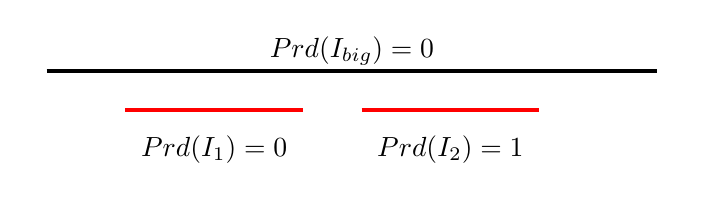
\begin{tikzpicture}[scale=0.5]
	
	\node at (0,0.5) {$Prd(I_{big}) = 0$};
	\node[draw=none] (I1a) at (-8,0) {$ $};
	\node[draw=none] (I1b) at (8,0) {$ $};
	\draw[line width=0.5mm] (I1a) -- (I1b);

	\node[draw=none] (I5a) at (-6,-1) {$ $};
	\node[draw=none] (I5b) at (-1,-1) {$ $};
	\node at (-3.5,-2) {$Prd(I_{1})=0$};
	\draw[color=red,line width=0.5mm] (I5a) -- (I5b);

 \node[draw=none] (I6a) at (0,-1) {$ $};
	\node[draw=none] (I6b) at (5,-1) {$ $};
	\node at (2.5,-2) {$Prd(I_{2})=1$};
	\draw[color=red,line width=0.5mm] (I6a) -- (I6b);

	\end{tikzpicture} 
        \caption{Instance of theorem \ref{theo:unw-naive-neg}.}
        \label{fig:neg-unit-irrev}
    \end{figure}
\end{proof}

\begin{corollary}
    Algorithm Naive is optimal for unit weights in the model of irrevocable acceptances.
\end{corollary}
Boyar et al. \cite{boyar2023online} were the first to consider the problem of interval selection with unit weights and irrevocable decisions, and they get the same (syntactically) performance, using a different algorithm, and a different set of predictions and error measure. In comparing our result to theirs, we note that our predictions are information theoretically strictly weaker than theirs\footnote{Their predictions consist of the entire input instance given in advance.}, and can in fact easily be extracted from theirs, allowing our algorithms to operate in their model. Furthermore, their predictions-following algorithm is enhanced with a \textit{greedy} aspect in order to achieve this optimal performance. As we will see in section \ref{section:exp}, experimental results on real-world data suggest that for some error ranges, pure \textit{greediness} is arguably a more important attribute than the use of predictions for getting a good solution, and the combination of both in the context of revocable acceptances works best.\\\\

We will now show that with \textbf{proportional weights}, algorithm \texttt{Naive} achieves the same performance bounds as in the case of unit weights.

\begin{theorem}
Algorithm Naive achieves $ALG \geq OPT - \eta$ for interval selection with proportional weights.
    \label{theo:prop-naive-pos}
\end{theorem}
\begin{proof}
        Without loss of generality, we assume integral lengths of intervals, and later explain how to generalize to real lengths. We discretize the weight of intervals into weight units, and define a weight element $w$ for each unit of weight. Let $W_{I} = \{w_{1},...,w_{w(I)}\}$ be the set of weight elements corresponding to the weight of interval $I$, with $W_{I} \cap W_{J} = \emptyset$ for any two distinct intervals $I,J$ . Let $W_{opt} = \bigcup_{I\in OPT}W_{I}$, and $W_{alg} = \bigcup_{I\in ALG}W_{I}$. The sets $H$ and $H_{I}$ are defined as for the unweighted algorithms. Lastly, let $C_{opt}(I)$ be the set of optimal intervals in $OPT$ that conflict with interval $I$.\\\\
    We argue for the existence of an injective mapping $F: W_{opt} \rightarrow W_{alg} \cup H$ as follows: Let $I_{opt}$ be an optimal interval. If $I_{opt}$ is taken by the algorithm, we map the elements of $W_{I_{opt}}$ to their corresponding elements in $W_{alg}$. If $I_{opt}$ is not taken by the algorithm, there are two cases. The first case is that $I_{opt}$ did not conflict with any interval in the solution, but $Prd(I_{opt}) = 0$. In this case, we know that $\eta(I_{opt}) = |H_{I_{opt}}| = w(I_{opt})$, and we can map the weight elements of $I_{opt}$ to error elements in $H_{I_{opt}}$.\\\\
    The other case is that $I_{opt}$ conflicted with at least one interval in the solution. Let that conflicting interval be $I_{c}$. It could also be that $Prd(I_{opt}) = 0$, and $H_{I_{opt}}$ would have error elements we can use, but we will assume the worst case of $Prd(I_{opt}) = 1$. In this case, it could be  $|W_{I_{opt}}| >  |H_{I_{c}}|$, and we cannot map the weight elements to error elements exclusively. We can, however, map the optimal weight elements, to elements in $H_{I_{c}} \cup W_{I_{c}}$. To see that there will always be sufficiently many unmapped elements, notice that $|H_{I_{c}} \cup W_{I_{c}}| \geq |\bigcup_{I \in C_{opt}(I_{c})}W_{I}|$. This is because $|H_{I_{c}}| = |\bigcup_{I \in C_{opt}(I_{c})}W_{I}| - |W_I|$, and $W_{I_c} \cap H_{I_c} = \emptyset$ always holds. We conclude that $|W_{alg}| + |H| \geq |W_{opt}|$, and we get the desired bound.\\\\
    To adapt the proof to real lengths, instead of considering sets of error and weight elements, we can define a transport plan using two transport matrices $H$ and $W$ of size $OPT\times ALG$. $H_{ij}$ (respectively $W_{ij}$) corresponds to the (real) amount of weight, or mass, mapped from $I_i \in OPT$ to the amount of error (resp. weight) introduced by $I_j \in ALG$. We can define these matrices such that for $1 \leq i \leq OPT$, $\sum_{1\leq j \leq ALG} H_{ij} + W_{ij} = w(I_i)$, for $1\leq j \leq ALG$, we have that $\sum_{1\leq i \leq OPT}H_{ij} \leq \eta(I_j)$ and $\sum_{1\leq i \leq OPT}W_{ij} \leq w(I_j)$.
\end{proof}
\begin{theorem}
For every deterministic algorithm, there exist a proportional weights instance and predictions, such that $ALG = OPT - \eta$.
    \label{theo:prop-naive-neg}
\end{theorem}
\begin{proof}
    Let $I_{1}$ arrive first with $Prd(I_{1}) = 0$. If the algorithm doesn't accept $I_{1}$, no more intervals arrive, and we have that $ALG = 0$, $OPT = w(I_{1})$, and $\eta = w(I_{1})$. If the algorithm accepts $I_{1}$, let two intervals $I_2$ and $I_3$ arrive next, with $w(I_2) = w(I_1)$, $Prd(I_2) = 1$, $w(I_3) = 2w(I_1)$ and $Prd(I_3) = 0$. In this case we have $ALG = w(I_1)$, $OPT = 3w(I_1)$, and $\eta = \eta(I_3) = 2w(I_1)$. In both cases the equality holds. One can repeat this construction for an asymptotic result.
\end{proof}

    \begin{figure}
	\centering
	
	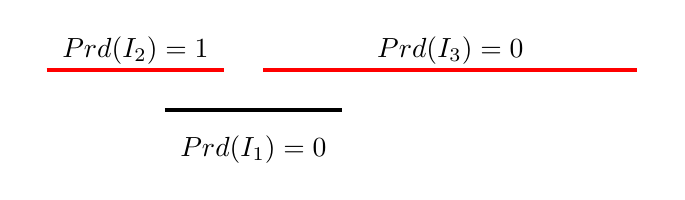
\begin{tikzpicture}[scale=0.5]

	\node at (-5,-2) {$Prd(I_{1}) = 0$};
	\node[draw=none] (I1a) at (-7.5,-1) {$ $};
	\node[draw=none] (I1b) at (-2.5,-1) {$ $};
	\draw[line width=0.5mm] (I1a) -- (I1b);
	
	
	%\node[draw=none] (d1) at (-3,-1) {$\rvdots$};

	
	\node[draw=none] (I3a) at (-10.5,0) {$ $};
	\node[draw=none] (I3b) at (-5.5,0) {$ $};
	\node at (-8,0.5) {$Prd(I_{2}) = 1$};
	\draw[color=red,line width=0.5mm] (I3a) -- (I3b);
	
	\node[draw=none] (I4a) at (-5,0) {$ $};
	\node[draw=none] (I4b) at (5,0) {$ $};
	\node at (0,0.5) {$Prd(I_{3}) = 0$};
	\draw[color=red,line width=0.5mm] (I4a) -- (I4b);

	\end{tikzpicture} 
	\caption{Instance of Theorem \ref{theo:prop-naive-neg}, with $w(I_2) = w(I_1), w(I_3) = 2w(I_1)$.}\label{fig:prop-neg-no-rev}
\end{figure}

\begin{corollary}
 Algorithm Naive is optimal for proportional weights in the model of irrevocable acceptances.
\end{corollary}
%%%%%%%%%%%%%%%%%%%%%%%%%%%%%%%%%%%%%%%%%%%%%%%%%%%%%%%%%%%%%%%%%%%%%%%%
\section{Revocable Acceptances}\label{section:rev}
Given the difficulty of the problem(s) in the conventional online model, we now consider the case where acceptances are revocable, but rejections are final, a relaxation of the model that is commonly studied for the problem of interval selection. A new interval can now always be accepted by displacing any intervals in the solution conflicting with it. For unit weights, Borodin and Karavasilis \cite{borodin2023any} give an optimal algorithm that is $2k$-competitive, where $k$ is the number of distinct interval lengths. We will refer to this algorithm of \cite{borodin2023any} as the \textit{BK2K} algorithm. \textit{BK2K} is a greedy algorithm, always accepting a new interval when there is no conflict, and whenever a conflict exists, the new interval is accepted only if it is properly included in an interval currently in the solution. We use that as the base logic for our predictions algorithm, and add one more replacement rule, which accepts a new interval $I$ that is only involved in partial conflicts, if $Prd(I) = 1$. Furthermore, an interval accepted by that rule gets marked, to make sure it cannot be replaced by that rule again. We call this algorithm \texttt{Revoke-Unit} \ref{alg:unw-revoke}. Interestingly, this rule of locally \textit{following the predictions once}, suffices to give us $1$-consistency.




\begin{algorithm}
\caption{\texttt{Revoke-Unit}}\label{alg:unw-revoke}
\begin{algorithmic}
\State $M \gets \emptyset$ \Comment{Set of marked intervals}
\State $S \gets \emptyset$ \Comment{Solution set}
\State On the arrival of $I$:
\State $I_{s} \gets $ Set of intervals currently in the solution conflicting with $I$
\If{$I_{s} = \emptyset$ or ($I_{s}=\{I'\}$ and $I \subset I'$)}
    \If{ $I' \in M$}
        \State $M \gets M \cup \{I\}$
    \EndIf
    \State $S \gets S \cup \{I\} \setminus \{I'\} $\Comment{Take $I$ and discard $I'$ if necessary}
\ElsIf{$I$ is only involved in partial conflicts \textbf{and} $Prd(I) = 1$ \textbf{and} $I_{s} \cap M = \emptyset$}
    \State $S \gets S \cup \{I\} \setminus I_s $\Comment{Take $I$ and discard conflicting intervals}
    \State $M \gets M \cup \{I\}$
\EndIf
\end{algorithmic}
\end{algorithm}
%Algorithm \ref{alg:unw-revoke} is a greedy algorithm that uses the same replacement rule (replace when new interval entirely subsumed by existing one) as the optimal $2k$ online algorithm, but has one additional replacement rule for partial conflicts. If the newly arrived interval is only involved in partial conflicts (can only be one or two such conflicts at most), the prediction says it's optimal, and the existing intervals it conflicts with are unmarked (have not been involved in a partial-conflict replacement in the past), then it accepts the new interval. {\color{red} Talk about how follow-the-prediction-ONCE works is the main idea, and suffices for 1-consistency. Also mention the BK2K notation.}

\begin{theorem}
    Algorithm \ref{alg:unw-revoke} achieves $ALG \geq OPT - \eta$.
\end{theorem}
\begin{proof}
    We follow the same approach as in the proof of Theorem \ref{theo:unw-naive-pos}, mapping optimal intervals to intervals taken by the algorithm, and to error. The main difference is that because of revoking, this mapping might be redefined throughout the execution of the algorithm. As before, we let $H$ be the set of error elements, and $H_{I} \subseteq H$ be the set of error elements introduced by $\eta(I)$. Let $I_{opt}$ be an optimal interval. We will define an injective mapping $F: OPT \rightarrow ALG \cup H$ as follows: If $I_{opt}$ is taken by the algorithm, it is initially mapped onto itself. If $I_{opt}$ is later replaced, it must be because of a partial conflict (w.l.o.g. no interval is subsumed by an optimal interval) with a new interval $I'$ with $Prd(I') = 1$. In this case, $I_{opt}$ will be mapped to an error element in $H_{I'}$, or if no further optimal intervals that conflict with $I$ are yet to arrive, it will be mapped to $I$. In both, subcases it will never be remapped.\\
    Consider now the case of $I_{opt}$ being rejected upon arrival. This can only happen if it is involved in (at most two) partial conflicts. There are two possible cases. The first case is that $Prd(I_{opt}) = 0$, and therefore $|H_{I_{opt}}| = 1$, in which case we map $I_{opt}$ to the error element of its own prediction. The second case is that $Prd(I_{opt}) = 1$, but at least one of the conflicting intervals was marked. Let $I_{c}$ be one of the marked, partially conflicting intervals. If $I_{c}$ was marked by being taken through a partial-conflict replacement, it means that $Prd(I_{c}) = 1$, and $|H_{I_{c}} \cup \{I_c\}| > 0$, in which case we can map $I_{opt}$ to an element $h_{c} \in H_{I_{c}}\cup \{I_c\}$.\\
    If $I_{c}$ was instead marked by a proper-inclusion-replacement, we trace the original interval that got marked through a partial-conflict-replacement. Call that interval $I^{'}_{c}$. It holds that $I^{'}_{c}$ conflicts with $I_{c}$, and therefore also conflicts with $I_{opt}$. Moreover, for $I^{'}_{c}$ to have been accepted, it must be that $Prd(I^{'}_{c})=1$ and $|H_{I^{'}_{c}} \cup \{I^{'}_{c}\}|>0$. In this case, we map $I_{opt}$ to an element $h_{c'} \in H_{I^{'}_{c}} \cup \{I^{'}_{c}\}$. In conclusion, we have that $ALG + |H| \geq OPT$, and we get the desired bound.
\end{proof}

We note that the performance of algorithm \ref{alg:unw-revoke} on the instance of Theorem \ref{theo:unw-naive-neg} is exactly equal to $OPT - \eta$, and we get the following lemma.

\begin{lemma}
    The performance of algorithm \ref{alg:unw-revoke} cannot be better than $OPT-\eta$.
\end{lemma}

We next show that the robustness of algorithm \texttt{Revoke-Unit} nearly matches the optimal online guarantee.

\begin{theorem} \label{theo:unw-rev-robust}
    With at most $k$ distinct interval lengths, algorithm \ref{alg:unw-revoke} is $(2k+1)$-robust.
\end{theorem}
\begin{proof}
    We use a charging argument and show that an interval taken by the algorithm can be charged by at most $2k+1$ optimal intervals. As soon as an optimal interval arrives, we map it to an interval already taken by the algorithm or itself. When an interval is replaced during the execution, all optimal intervals charged to it up to that point, will now be charged to the new interval that was accepted. We build upon the proof of Theorem 3.2 in \cite{borodin2023any}. In the case of the \textit{BK2K} algorithm (\cite{borodin2023any}), it is true that for every predecessor trace $\mathcal{P}$, and consecutive intervals $(I_i,I_{i+1}) \in \mathcal{P}$, $\Phi(I_{i+1}) \leq \Phi(I_i) + 2$, and the length of every predecessor trace is at most $k$. While the former is still true for algorithm \texttt{Revoke-Unit}, the latter is not, and that is because we have an additional replacement rule. However, we argue that for every $I_i \in \mathcal{P}$, if $I_j,\; j > i$ is the next interval in the trace that was accepted through proper-inclusion, it is true that $TC(I_j) \leq TC(I_i) + 3$.\\
    
    Figure \ref{fig:pcr-charge} shows how to maximize charge on the event of a partial-conflict replacement. Before being replaced by a partially-conflicting interval, $I_{1}$ can be directly charged by at most two optimal intervals ($I^{1}_{opt}, I^{2}_{opt}$), one on each side. After $I_{2}$ replaces $I_{1}$, it can also be directly charged by two optimal intervals, but only if $I^{2}_{opt}$ was not charged to $I_{1}$ earlier. In other words, if $I_{2}$ is directly charged by two new intervals, it means that $I_{1}$ was directly charged by at most one, concluding that $\Phi(I_2) \leq TC(I_1) + 3$.

    \begin{figure}[H]
	\centering
	
	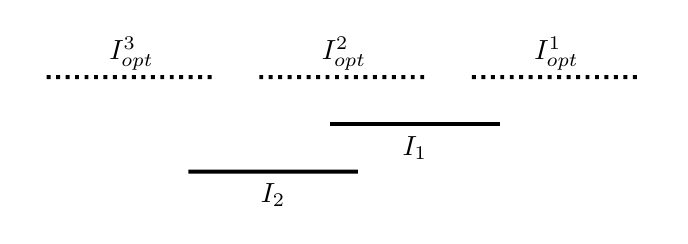
\begin{tikzpicture}[scale=0.6]

	\node at (-5,-1.5) {$I_{2}$};
	\node[draw=none] (I1a) at (-7,-1) {$ $};
	\node[draw=none] (I1b) at (-3,-1) {$ $};
	\draw[line width=0.5mm] (I1a) -- (I1b);
	
	
	%\node[draw=none] (d1) at (-3,-1) {$\rvdots$};

	\node[draw=none] (I2a) at (-5.5,1) {$ $};
	\node[draw=none] (I2b) at (-1.5,1) {$ $};
	\node at (-3.5,1.5) {$I^{2}_{opt}$};
	\draw[dotted,line width=0.5mm] (I2a) -- (I2b);
	
	\node[draw=none] (I3a) at (-10,1) {$ $};
	\node[draw=none] (I3b) at (-6,1) {$ $};
	\node at (-8,1.5) {$I^{3}_{opt}$};
	\draw[dotted,line width=0.5mm] (I3a) -- (I3b);
	
	\node[draw=none] (I4a) at (-4,0) {$ $};
	\node[draw=none] (I4b) at (0,0) {$ $};
	\node at (-2,-0.5) {$I_{1}$};
	\draw[line width=0.5mm] (I4a) -- (I4b);
	
	\node[draw=none] (I5a) at (-1,1) {$ $};
	\node[draw=none] (I5b) at (3,1) {$ $};
	\node at (1,1.5) {$I^{1}_{opt}$};
	\draw[dotted,line width=0.5mm] (I5a) -- (I5b);

	\end{tikzpicture} 
	\caption{Maximum charge through partial-conflict replacement.}\label{fig:pcr-charge}
\end{figure}

Finally, notice that because the mark of an interval carries over when it is replaced, the event of a partial-conflict replacement can occur at most once in each predecessor trace,
and excluding at most one subsequence $(I_i, I_r, I_j) \in \mathcal{P}$ where $TC(I_j) \leq TC(I_i) + 3$, it holds that for $(I_b,I_{b+1}) \in \mathcal{P}$, $\Phi(I_{b+1})\leq \Phi(I_b) + 2$, giving us a worst case competitive ratio of $2k+1$. 
\end{proof}

\begin{corollary}
    With at most $k$ distinct interval lengths, and predictions with total error $\eta$, Algorithm Revoke-Unit achieves $ALG \geq \max\{OPT-\eta , \frac{OPT}{2k+1}\}$.
\end{corollary}

Notice how we can choose not to carry over the mark when proper-inclusion replacement occurs, and get a $3k$-robust algorithm. Such an algorithm is prone to follow the prediction more often, and it can outperform \texttt{Revoke-Unit} for some small values of error caused by adversarial predictions.\\\\
We now look at the case of proportional weights. In the conventional online setting, Garay et al. \cite{garay1997efficient} give a $2\phi + 1  \approx 4.236-$competitive algorithm, while Tomkins \cite{tomkins1995lower} gives a matching lower bound. They call their optimal algorithm \texttt{LR} (for \textit{length of route}), and we include it here for completeness. Unlike the case of unit weights, we now want to accept intervals that occupy as much of the line as possible. Algorithm \texttt{LR} works greedily by always accepting a new interval with no conflicts, and when there are conflicts, it accepts the new interval if its length is at least $\phi$ times greater than the largest conflicting interval. More generally, using parameter $\beta \geq \phi$, we have the following lemma:
\begin{lemma}[Garay et al. \cite{garay1997efficient}]
    Algorithm \texttt{LR} with parameter $\beta \geq \phi$ is $(2\beta + 1)$-competitive for the problem of interval selection with proportional weights.
\end{lemma}
\begin{algorithm}
\caption{LR \cite{garay1997efficient}}\label{alg:garay_prop}
\begin{algorithmic}
\State Parameter $\beta = \phi$ \Comment{optimal value for parameter $\beta$}
\State On the arrival of $I$:
\State $I_{s} \gets $ Set of intervals currently in the solution conflicting with $I$
\If{ $w(I) > \beta \cdot \max\{w(J)\; : \; J\in I_s\}$}
    \State Accept $I$ and displace conflicts
    \State Return
\EndIf
\end{algorithmic}
\end{algorithm}
Instead of using algorithm \texttt{LR} as the base of our predictions algorithm, we consider a slightly modified version, which we refer to as \texttt{LR$'$}, and which compares the weight of the new interval to the sum of the weights of the conflicting intervals, instead of looking only at the longest interval. Although we do not know the exact performance of algorithm \texttt{LR$'$} in the online model, we conjecture it is also $(2\phi + 1)$-competitive.\\\\
In trying to utilize predictions in the case of proportional weights, we first make the following observations:
\begin{observation}
    $1$-consistency is unattainable while maintaining bounded robustness.
\end{observation}
\begin{proof}
    To be $1$-consistent, the algorithm must be able to replace an interval with an arbitrarily smaller one that is part of the optimal solution. The adversary could then stop the instance, forcing arbitrarily bad robustness.
\end{proof}

\begin{observation}
    In order to have bounded robustness, it must be that a new interval that is sufficiently large (small\footnote{More accurately, an interval reducing ALG sufficiently much. }) must always be accepted (rejected).
\end{observation}

\begin{definition}[$\alpha-$increasing]
    An $\alpha$-increasing algorithm never accepts a new conflicting interval
that is less than $\alpha$ times the longest interval it conflicts with.
\end{definition}
\begin{lemma}
    An $\alpha$-increasing algorithm (greedy or non-greedy), cannot be better than $(2\alpha +1)$-consistent.
\end{lemma}
\begin{proof}
    Let an interval $I_1$ arrive first. Let $I_2$ and $I_3$ be intervals that partially conflict with $I_1$ on either side, and $w(I_2) = w(I_3) = \alpha \cdot w(I_1) - \epsilon$. Let $I_4$ with $w(I_4) = w(I_1)-2\epsilon$ be an interval that is fully subsumed by $I_4$. This instance is depicted in figure \ref{fig:neg-alpha-increasing}. The algorithm will never replace $I_1$, while the optimal solution is made of $\{I_2,I_3,I_4\}$.
    \begin{figure}[h] % Adjust the width as needed
        \centering
        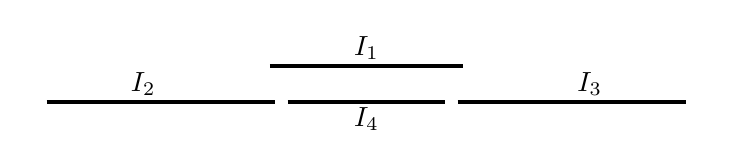
\begin{tikzpicture}[scale=0.45]
	
	\node at (0,0.5) {$I_1$};
	\node[draw=none] (I1a) at (-3,0) {$ $};
	\node[draw=none] (I1b) at (3,0) {$ $};
	\draw[line width=0.5mm] (I1a) -- (I1b);

 \node at (-6.3,-0.5) {$I_2$};
	\node[draw=none] (I2a) at (-9.3,-1) {$ $};
	\node[draw=none] (I2b) at (-2.3,-1) {$ $};
	\draw[line width=0.5mm] (I2a) -- (I2b);

  \node at (6.3,-0.5) {$I_3$};
	\node[draw=none] (I2a) at (2.3,-1) {$ $};
	\node[draw=none] (I2b) at (9.3,-1) {$ $};
	\draw[line width=0.5mm] (I2a) -- (I2b);

	\node[draw=none] (I5a) at (-2.5,-1) {$ $};
	\node[draw=none] (I5b) at (2.5,-1) {$ $};
	\node at (0,-1.5) {$I_{4}$};
	\draw[line width=0.5mm] (I5a) -- (I5b);

	\end{tikzpicture} 
        \caption{Consistency bound for $\alpha$-increasing algorithms.}
        \label{fig:neg-alpha-increasing}
    \end{figure}
\end{proof}
Algorithm \texttt{LR} is a $\phi$-increasing algorithm, while the algorithm by Woeginger \cite{woeginger1994line} for the real-time model is $2$-increasing. Our predictions algorithm \ref{alg:prop-revoke2} \texttt{Revoke-Proportional} is $1$-increasing. The algorithm works like \texttt{LR$'$}, with one additional replacement rule that accepts a new interval that is predicted to be optimal, even if it is not sufficiently larger than what it conflicts with. More precisely, if a new interval is predicted to be optimal and is at least as big as the sum of the weights of the intervals it conflicts with, and none of the conflicting intervals were predicted to be optimal, it will be accepted through the predictions rule. The algorithm takes a parameter $\lambda > 1$, which can be thought of as an indicator of how much the predictions are trusted. As $\lambda$ increases, the consistency bound improves.

\begin{algorithm}
\caption{\texttt{Revoke-Proportional} {\hfil Parameter: $\lambda > 1$ }}\label{alg:prop-revoke2}
\begin{algorithmic}
\State On the arrival of $I$:
\State $I_{s} \gets $ Set of intervals currently in the solution conflicting with $I$
\State Let $w_c = \sum_{J \in I_s} w(J)$ \Comment{Total weight of conflicting intervals}
\If{ $w(I) \geq \lambda\cdot w_c$} \Comment{Main replacement rule}
    \State Accept $I$ and displace conflicts
    \State Return
\ElsIf{$Prd(I) = 1$} \Comment{Predictions rule} 
    \If{($w(I) \geq w_c$ and $|\{J: J \in I_s \text{ and }Prd(J)=1\}| = \emptyset$)} 
    \State Accept $I$ and displace conflicts
    \State Return
    \EndIf
\EndIf
\end{algorithmic}
\end{algorithm}

\begin{theorem}
    Algorithm Revoke-Proportional is $\frac{3\lambda}{\lambda -1}$-consistent.\label{theo:prop-consistent}
\end{theorem}
\begin{proof}
We consider the optimal solution $OPT$ consistent with the fully accurate predictions. We will show that throughout the execution of the algorithm, we have that $\Phi(I) \leq \mu \cdot w(I)$, for every $I$ in the current solution. In the end, we have that $\sum_{I\in ALG} \Phi(I) = OPT$, giving us the $\mu$-consistency of the algorithm.\\\\
As in the proof of Theorem \ref{theo:unw-rev-robust}, we consider the notions of \textit{transfer charge} ($TC$), and \textit{direct charge} ($DC$). We can express $\Phi(I) = TC(I) + DC(I)$. A transfer charge occurs whenever accepting a new interval $I$ replaces intervals currently in the solution. In that case, the total charge of those conflicting intervals is passed on as transfer charge to $I$. Any additional charge to $I$ after its acceptance is through direct charge, namely rejection of subsequent optimal intervals conflicting with $I$. We will write $DC_J(I)$ to denote the amount of direct charge from interval $J$ to interval $I$. Whenever an optimal interval is accepted, we consider its weight being directly charged to itself, and it cannot be directly charged again.\\\\
Whenever an optimal interval is rejected upon arrival, we charge its weight to the intervals it conflicts with, with its weight being distributed to all its conflicting intervals, in proportion to their weight. Specifically, let $I_o$ be the newly arrived optimal interval that is rejected, and $I_s$ denote the set of conflicting intervals. Each interval $J \in I_s$ is directly charged $DC_{I_o}(J)=w(I_o) \frac{w(J)}{w_c}\leq w(I_o)$. Furthermore, for an optimal interval to have been rejected, it must be that even the predictions rule failed, and because the predictions are accurate, it must have failed because $w(I_o) < w_c$. Because of this, we get that $w(I_o) \frac{w(J)}{w_c} \leq w(J)$, and therefore $DC_{I_o}(J)\leq\min\{w(I_o),w(J)\}$. An interval $I \in ALG$ can be directly charged by at most three different types of optimal intervals: 1) smaller intervals that are subsumed by it, 2) an optimal interval partially conflicting on the left, and 3) an optimal interval partially conflicting on the right.
In the case of smaller optimal intervals subsumed by $I$, the total amount of direct charge from those intervals can be at most $w(I)$. Given that each of the two possible partially conflicting intervals can directly charge $I$ at most $w(I)$, we conclude that for every $I\in ALG$:
\begin{equation}
\label{dc-bound}
    DC(I) \leq 3w(I)
\end{equation}
We omitted the case where the rejected optimal interval subsumes $I$, because in that case $DC(I) = w(I)$ and \ref{dc-bound} holds trivially. We now focus on the total amount of charge on any interval $I\in ALG$. Let:
$$\mu = \frac{3\lambda}{\lambda - 1}$$
We want to make sure that throughout the execution of the algorithm, $\Phi(I) \leq \mu \cdot w(I)$. Before any interval is accepted through replacement, intervals in the solution could have only been directly charged through rejected optimal intervals, and because of \eqref{dc-bound}, and the fact that $\lambda > 1$, our desired bound holds. We now consider all the cases of an interval being accepted through replacement.\\\\
\underline{Case $1$}: $I$ is an optimal interval and it is accepted through the predictions rule. In this case we have that $DC(I) = w(I)$, and we need to look at $TC(I)$. Let $L_c$ and $R_c$ denote the intervals (if any) that $I$ is partially conflicting with on the left and on the right respectively, and let $M_c$ denote the set of intervals that $I$ subsumes. We know that all of these conflicting intervals are not optimal, and they were accepted through the algorithm's main rule. First, notice that for all $J\in M_c$, $DC(J) = 0$, and $\Phi(J) = TC(J) \leq \frac{\mu}{\lambda} \cdot w(J)$. Moreover, $L_c$ and $R_c$ had not yet been directly charged by a partially conflicting optimal interval on one side, and therefore we have that $\Phi(L_c) \leq \frac{\mu}{\lambda}\cdot w(L_c) + 2w(L_c)$, and similarly $\Phi(R_c) \leq \frac{\mu}{\lambda}\cdot w(R_c) + 2w(R_c)$.\\
Putting everything together:
\[
\begin{aligned}
    TC(I) &= \sum_{J\in M_c} \Phi(J) + \Phi(L_c) + \Phi(R_c) \\
     & \leq \frac{\mu}{\lambda}\cdot w_c + 2(w(L_c) + w(R_c))\\
     & \leq \left(\frac{\mu}{\lambda} + 2\right)w_c\\
     &\leq \left(\frac{\mu}{\lambda} + 2\right)w(I)
\end{aligned}
\]
The last inequality being true from the fact that the main predictions rule is satisfied. Given also that $DC(I) = w(I)$, we get that $\Phi(I) \leq (\frac{\mu}{\lambda} + 2)w(I) + w(I) = (\frac{\mu}{\lambda} + 3)w(I)$. With our choice of $\mu$, we have:
\[\begin{aligned}
    \Phi(I) &\leq \left(\frac{\frac{3\lambda}{\lambda - 1}}{\lambda} + 3 \right)w(I) \\
    &= \left(\frac{3\lambda}{\lambda -1}\right)w(I)\\\\
\end{aligned}\]
\underline{Case $2$}: $I$ is an optimal interval and it is accepted through the algorithm's main rule. This is similar to case 1, with $DC(I) = w(I)$ and $w(I)\geq \lambda \cdot w_c$. The same analysis gives us $TC(I)\leq \left( \frac{\mu}{\lambda} + 2 \right)\frac{w(I)}{\lambda}$, and because $\lambda > 1$, the same bound holds.\\\\
\underline{Case $3$}: $I$ is not an optimal interval and it is accepted through the algorithm's main rule. In this case we have that $DC(I) \leq 3w(I)$, and we get that
\[\begin{aligned}
    \Phi(I) & \leq \sum_{J\in I_s} \Phi(J) + 3w(I)\\
    & \leq \frac{\mu}{\lambda}\cdot w(I) + 3w(I)\\
    & = \left(\frac{3\lambda}{\lambda -1}\right)w(I)
\end{aligned}\]
In conclusion, we have that throughout the execution of the algorithm, for $I \in ALG$, $\Phi(I)\leq \frac{3\lambda}{\lambda - 1}w(I)$, and therefore $\frac{OPT}{ALG} \leq \frac{3\lambda}{\lambda - 1}$. 
\end{proof}
\vspace{0.5cm}
We see that as $\lambda \rightarrow \infty$, the algorithm's consistency goes to $3$. We now look at the robustness of algorithm \texttt{Revoke-Proportional}.\\
\begin{theorem}
    Algorithm Revoke-Proportional is $\frac{4\lambda^2 + 2\lambda}{\lambda -1}$-robust.
\end{theorem}
\begin{proof}
    The argument is similar to the proof of Theorem \ref{theo:prop-consistent}. Both \textit{direct}, and \textit{transfer} charging work the same way as before. Let $\mu = \frac{2\lambda^2 +3\lambda + 1}{\lambda -1 }$, and $\delta = 2\lambda + 1$. We will show that that for every $I \in ALG$, $\Phi(I)\leq (\mu + \delta)\cdot w(I)=\frac{4\lambda^2 + 2\lambda}{\lambda -1}w(I)$.\\\\
    Notice first that the upper bound on direct charging is not as good as before. More precisely, with $I_o$ being a newly arrived optimal interval that will be rejected and $I_s$ being its conflicting intervals currently in the solution, we have that for every $J\in I_s$, $DC_{I_o}(J)= w(I_o)\frac{w(J)}{w_c}\leq \lambda \cdot w(J)$. More generally, $DC_{I_o}(J) \leq \min\{w(I_o),\lambda\cdot w(J)\}$. As before, given the three different possible types of conflicts, we have that:
    \begin{equation}
        DC(I) \leq (2\lambda + 1)w(I)
    \end{equation}
    We can now bound the total amount of charge on every interval in the algorithm's solution, throughout its execution. Before any replacement happens, the bound $\Phi(I) \leq (\mu + \delta)\cdot w(I)$ holds trivially.\\\\
    \underline{Case $1$}: Interval $I$ is accepted through the algorithm's main rule. We get that:
    \[\begin{aligned}
        \Phi(I) &\leq (\mu + \delta)\cdot w_c + (2\lambda + 1)\cdot w(I)\\
        & \leq (\mu + \delta)\cdot \frac{w(I)}{\lambda} + (2\lambda + 1)\cdot w(I)\\
        & = \left(\frac{\mu + \delta}{\lambda} + 2\lambda + 1\right)w(I)\\
        & = \left( \frac{\frac{4\lambda^2 +2\lambda}{\lambda-1}+2\lambda^2 + \lambda}{\lambda} \right)w(I)\\
        & = \mu \cdot w(I)
    \end{aligned}\]
\underline{Case $2$}: Interval $I$ is accepted through the algorithm's predictions rule. Notice that in this case, all conflicting intervals must have been accepted through the main rule, and not the predictions rule. Because of this, as we showed in case $1$, for every $J\in I_s$, it holds that $\Phi(J) \leq \mu\cdot w(J)$. This helps us bound the amount of transfer charge to interval $I$.
\[\begin{aligned}
    \Phi(I) &\leq \mu \cdot w_c + (2\lambda + 1)\cdot w(I)\\
    & \leq \mu \cdot w(I) + (2\lambda + 1)\cdot w(I) \\
    & = (\mu + \delta)\cdot w(I)
\end{aligned}\]
To summarize, we have shown that in the worst case, $\Phi(I) \leq (\mu + \delta)\cdot w(I)$ for every $I\in ALG$. This concludes the proof.
\end{proof}

\begin{figure*}[t!]
\centering
\caption{\texttt{NASA-iPSC} dataset.} (a) Unit \& Irrevocable, (b) Unit \& Revoking, (c) Proportional \& Irrevocable, (d) Proportional \& Revoking
\includegraphics[width=\textwidth]{exp_pics/nasa/nasa_combined_ann.png}
\label{fig:nasa_exps}
\end{figure*}
\begin{figure*}[t!]
\centering
\caption{\texttt{CTC-SP2} dataset.}
\includegraphics[width=\textwidth]{exp_pics/ctc/ctc_combined_ann.png}
\label{fig:ctc_exps}
\end{figure*}

We note that for $\lambda > \frac{2+\sqrt{5}}{\sqrt{5} -1}\approx 3.42 $, the consistency of our algorithm is already better than $2\phi + 1$, and $22.15$-robust. We have shown we can get consistency better than the online bound of \texttt{LR}, while maintaining bounded robustness. We believe further improvement on the bounds of \texttt{Revoke-Proportional} is possible, with an analysis that looks more closely at the dependence between direct and transfer charging.\\
One may also be able to further improve the algorithm by accepting an interval that is not as big as the sum of its conflicts, making the algorithm $a$-increasing with $a<1$. This would relax the predictions rule further, and make the algorithm more prone to bad choices caused by misleading predictions. In our experiments, we briefly discuss one such algorithm, which we call \texttt{Revoke-Prop-Half}, and which can accept a supposedly optimal interval even if it is half as big as its conflicts.







%%%%%%%%%%%%%%%%%%%%%%%%%%%%%%%%%%%%%%%%%%%%%%%%%%%%%%%%%%%%%%%%%%%%%%%%

\section{Experimental Results}\label{section:exp}
\section{Experiments}
\label{sec:experiments}
The experiments are designed to address two key research questions.
First, \textbf{RQ1} evaluates whether the average $L_2$-norm of the counterfactual perturbation vectors ($\overline{||\perturb||}$) decreases as the model overfits the data, thereby providing further empirical validation for our hypothesis.
Second, \textbf{RQ2} evaluates the ability of the proposed counterfactual regularized loss, as defined in (\ref{eq:regularized_loss2}), to mitigate overfitting when compared to existing regularization techniques.

% The experiments are designed to address three key research questions. First, \textbf{RQ1} investigates whether the mean perturbation vector norm decreases as the model overfits the data, aiming to further validate our intuition. Second, \textbf{RQ2} explores whether the mean perturbation vector norm can be effectively leveraged as a regularization term during training, offering insights into its potential role in mitigating overfitting. Finally, \textbf{RQ3} examines whether our counterfactual regularizer enables the model to achieve superior performance compared to existing regularization methods, thus highlighting its practical advantage.

\subsection{Experimental Setup}
\textbf{\textit{Datasets, Models, and Tasks.}}
The experiments are conducted on three datasets: \textit{Water Potability}~\cite{kadiwal2020waterpotability}, \textit{Phomene}~\cite{phomene}, and \textit{CIFAR-10}~\cite{krizhevsky2009learning}. For \textit{Water Potability} and \textit{Phomene}, we randomly select $80\%$ of the samples for the training set, and the remaining $20\%$ for the test set, \textit{CIFAR-10} comes already split. Furthermore, we consider the following models: Logistic Regression, Multi-Layer Perceptron (MLP) with 100 and 30 neurons on each hidden layer, and PreactResNet-18~\cite{he2016cvecvv} as a Convolutional Neural Network (CNN) architecture.
We focus on binary classification tasks and leave the extension to multiclass scenarios for future work. However, for datasets that are inherently multiclass, we transform the problem into a binary classification task by selecting two classes, aligning with our assumption.

\smallskip
\noindent\textbf{\textit{Evaluation Measures.}} To characterize the degree of overfitting, we use the test loss, as it serves as a reliable indicator of the model's generalization capability to unseen data. Additionally, we evaluate the predictive performance of each model using the test accuracy.

\smallskip
\noindent\textbf{\textit{Baselines.}} We compare CF-Reg with the following regularization techniques: L1 (``Lasso''), L2 (``Ridge''), and Dropout.

\smallskip
\noindent\textbf{\textit{Configurations.}}
For each model, we adopt specific configurations as follows.
\begin{itemize}
\item \textit{Logistic Regression:} To induce overfitting in the model, we artificially increase the dimensionality of the data beyond the number of training samples by applying a polynomial feature expansion. This approach ensures that the model has enough capacity to overfit the training data, allowing us to analyze the impact of our counterfactual regularizer. The degree of the polynomial is chosen as the smallest degree that makes the number of features greater than the number of data.
\item \textit{Neural Networks (MLP and CNN):} To take advantage of the closed-form solution for computing the optimal perturbation vector as defined in (\ref{eq:opt-delta}), we use a local linear approximation of the neural network models. Hence, given an instance $\inst_i$, we consider the (optimal) counterfactual not with respect to $\model$ but with respect to:
\begin{equation}
\label{eq:taylor}
    \model^{lin}(\inst) = \model(\inst_i) + \nabla_{\inst}\model(\inst_i)(\inst - \inst_i),
\end{equation}
where $\model^{lin}$ represents the first-order Taylor approximation of $\model$ at $\inst_i$.
Note that this step is unnecessary for Logistic Regression, as it is inherently a linear model.
\end{itemize}

\smallskip
\noindent \textbf{\textit{Implementation Details.}} We run all experiments on a machine equipped with an AMD Ryzen 9 7900 12-Core Processor and an NVIDIA GeForce RTX 4090 GPU. Our implementation is based on the PyTorch Lightning framework. We use stochastic gradient descent as the optimizer with a learning rate of $\eta = 0.001$ and no weight decay. We use a batch size of $128$. The training and test steps are conducted for $6000$ epochs on the \textit{Water Potability} and \textit{Phoneme} datasets, while for the \textit{CIFAR-10} dataset, they are performed for $200$ epochs.
Finally, the contribution $w_i^{\varepsilon}$ of each training point $\inst_i$ is uniformly set as $w_i^{\varepsilon} = 1~\forall i\in \{1,\ldots,m\}$.

The source code implementation for our experiments is available at the following GitHub repository: \url{https://anonymous.4open.science/r/COCE-80B4/README.md} 

\subsection{RQ1: Counterfactual Perturbation vs. Overfitting}
To address \textbf{RQ1}, we analyze the relationship between the test loss and the average $L_2$-norm of the counterfactual perturbation vectors ($\overline{||\perturb||}$) over training epochs.

In particular, Figure~\ref{fig:delta_loss_epochs} depicts the evolution of $\overline{||\perturb||}$ alongside the test loss for an MLP trained \textit{without} regularization on the \textit{Water Potability} dataset. 
\begin{figure}[ht]
    \centering
    \includegraphics[width=0.85\linewidth]{img/delta_loss_epochs.png}
    \caption{The average counterfactual perturbation vector $\overline{||\perturb||}$ (left $y$-axis) and the cross-entropy test loss (right $y$-axis) over training epochs ($x$-axis) for an MLP trained on the \textit{Water Potability} dataset \textit{without} regularization.}
    \label{fig:delta_loss_epochs}
\end{figure}

The plot shows a clear trend as the model starts to overfit the data (evidenced by an increase in test loss). 
Notably, $\overline{||\perturb||}$ begins to decrease, which aligns with the hypothesis that the average distance to the optimal counterfactual example gets smaller as the model's decision boundary becomes increasingly adherent to the training data.

It is worth noting that this trend is heavily influenced by the choice of the counterfactual generator model. In particular, the relationship between $\overline{||\perturb||}$ and the degree of overfitting may become even more pronounced when leveraging more accurate counterfactual generators. However, these models often come at the cost of higher computational complexity, and their exploration is left to future work.

Nonetheless, we expect that $\overline{||\perturb||}$ will eventually stabilize at a plateau, as the average $L_2$-norm of the optimal counterfactual perturbations cannot vanish to zero.

% Additionally, the choice of employing the score-based counterfactual explanation framework to generate counterfactuals was driven to promote computational efficiency.

% Future enhancements to the framework may involve adopting models capable of generating more precise counterfactuals. While such approaches may yield to performance improvements, they are likely to come at the cost of increased computational complexity.


\subsection{RQ2: Counterfactual Regularization Performance}
To answer \textbf{RQ2}, we evaluate the effectiveness of the proposed counterfactual regularization (CF-Reg) by comparing its performance against existing baselines: unregularized training loss (No-Reg), L1 regularization (L1-Reg), L2 regularization (L2-Reg), and Dropout.
Specifically, for each model and dataset combination, Table~\ref{tab:regularization_comparison} presents the mean value and standard deviation of test accuracy achieved by each method across 5 random initialization. 

The table illustrates that our regularization technique consistently delivers better results than existing methods across all evaluated scenarios, except for one case -- i.e., Logistic Regression on the \textit{Phomene} dataset. 
However, this setting exhibits an unusual pattern, as the highest model accuracy is achieved without any regularization. Even in this case, CF-Reg still surpasses other regularization baselines.

From the results above, we derive the following key insights. First, CF-Reg proves to be effective across various model types, ranging from simple linear models (Logistic Regression) to deep architectures like MLPs and CNNs, and across diverse datasets, including both tabular and image data. 
Second, CF-Reg's strong performance on the \textit{Water} dataset with Logistic Regression suggests that its benefits may be more pronounced when applied to simpler models. However, the unexpected outcome on the \textit{Phoneme} dataset calls for further investigation into this phenomenon.


\begin{table*}[h!]
    \centering
    \caption{Mean value and standard deviation of test accuracy across 5 random initializations for different model, dataset, and regularization method. The best results are highlighted in \textbf{bold}.}
    \label{tab:regularization_comparison}
    \begin{tabular}{|c|c|c|c|c|c|c|}
        \hline
        \textbf{Model} & \textbf{Dataset} & \textbf{No-Reg} & \textbf{L1-Reg} & \textbf{L2-Reg} & \textbf{Dropout} & \textbf{CF-Reg (ours)} \\ \hline
        Logistic Regression   & \textit{Water}   & $0.6595 \pm 0.0038$   & $0.6729 \pm 0.0056$   & $0.6756 \pm 0.0046$  & N/A    & $\mathbf{0.6918 \pm 0.0036}$                     \\ \hline
        MLP   & \textit{Water}   & $0.6756 \pm 0.0042$   & $0.6790 \pm 0.0058$   & $0.6790 \pm 0.0023$  & $0.6750 \pm 0.0036$    & $\mathbf{0.6802 \pm 0.0046}$                    \\ \hline
%        MLP   & \textit{Adult}   & $0.8404 \pm 0.0010$   & $\mathbf{0.8495 \pm 0.0007}$   & $0.8489 \pm 0.0014$  & $\mathbf{0.8495 \pm 0.0016}$     & $0.8449 \pm 0.0019$                    \\ \hline
        Logistic Regression   & \textit{Phomene}   & $\mathbf{0.8148 \pm 0.0020}$   & $0.8041 \pm 0.0028$   & $0.7835 \pm 0.0176$  & N/A    & $0.8098 \pm 0.0055$                     \\ \hline
        MLP   & \textit{Phomene}   & $0.8677 \pm 0.0033$   & $0.8374 \pm 0.0080$   & $0.8673 \pm 0.0045$  & $0.8672 \pm 0.0042$     & $\mathbf{0.8718 \pm 0.0040}$                    \\ \hline
        CNN   & \textit{CIFAR-10} & $0.6670 \pm 0.0233$   & $0.6229 \pm 0.0850$   & $0.7348 \pm 0.0365$   & N/A    & $\mathbf{0.7427 \pm 0.0571}$                     \\ \hline
    \end{tabular}
\end{table*}

\begin{table*}[htb!]
    \centering
    \caption{Hyperparameter configurations utilized for the generation of Table \ref{tab:regularization_comparison}. For our regularization the hyperparameters are reported as $\mathbf{\alpha/\beta}$.}
    \label{tab:performance_parameters}
    \begin{tabular}{|c|c|c|c|c|c|c|}
        \hline
        \textbf{Model} & \textbf{Dataset} & \textbf{No-Reg} & \textbf{L1-Reg} & \textbf{L2-Reg} & \textbf{Dropout} & \textbf{CF-Reg (ours)} \\ \hline
        Logistic Regression   & \textit{Water}   & N/A   & $0.0093$   & $0.6927$  & N/A    & $0.3791/1.0355$                     \\ \hline
        MLP   & \textit{Water}   & N/A   & $0.0007$   & $0.0022$  & $0.0002$    & $0.2567/1.9775$                    \\ \hline
        Logistic Regression   &
        \textit{Phomene}   & N/A   & $0.0097$   & $0.7979$  & N/A    & $0.0571/1.8516$                     \\ \hline
        MLP   & \textit{Phomene}   & N/A   & $0.0007$   & $4.24\cdot10^{-5}$  & $0.0015$    & $0.0516/2.2700$                    \\ \hline
       % MLP   & \textit{Adult}   & N/A   & $0.0018$   & $0.0018$  & $0.0601$     & $0.0764/2.2068$                    \\ \hline
        CNN   & \textit{CIFAR-10} & N/A   & $0.0050$   & $0.0864$ & N/A    & $0.3018/
        2.1502$                     \\ \hline
    \end{tabular}
\end{table*}

\begin{table*}[htb!]
    \centering
    \caption{Mean value and standard deviation of training time across 5 different runs. The reported time (in seconds) corresponds to the generation of each entry in Table \ref{tab:regularization_comparison}. Times are }
    \label{tab:times}
    \begin{tabular}{|c|c|c|c|c|c|c|}
        \hline
        \textbf{Model} & \textbf{Dataset} & \textbf{No-Reg} & \textbf{L1-Reg} & \textbf{L2-Reg} & \textbf{Dropout} & \textbf{CF-Reg (ours)} \\ \hline
        Logistic Regression   & \textit{Water}   & $222.98 \pm 1.07$   & $239.94 \pm 2.59$   & $241.60 \pm 1.88$  & N/A    & $251.50 \pm 1.93$                     \\ \hline
        MLP   & \textit{Water}   & $225.71 \pm 3.85$   & $250.13 \pm 4.44$   & $255.78 \pm 2.38$  & $237.83 \pm 3.45$    & $266.48 \pm 3.46$                    \\ \hline
        Logistic Regression   & \textit{Phomene}   & $266.39 \pm 0.82$ & $367.52 \pm 6.85$   & $361.69 \pm 4.04$  & N/A   & $310.48 \pm 0.76$                    \\ \hline
        MLP   &
        \textit{Phomene} & $335.62 \pm 1.77$   & $390.86 \pm 2.11$   & $393.96 \pm 1.95$ & $363.51 \pm 5.07$    & $403.14 \pm 1.92$                     \\ \hline
       % MLP   & \textit{Adult}   & N/A   & $0.0018$   & $0.0018$  & $0.0601$     & $0.0764/2.2068$                    \\ \hline
        CNN   & \textit{CIFAR-10} & $370.09 \pm 0.18$   & $395.71 \pm 0.55$   & $401.38 \pm 0.16$ & N/A    & $1287.8 \pm 0.26$                     \\ \hline
    \end{tabular}
\end{table*}

\subsection{Feasibility of our Method}
A crucial requirement for any regularization technique is that it should impose minimal impact on the overall training process.
In this respect, CF-Reg introduces an overhead that depends on the time required to find the optimal counterfactual example for each training instance. 
As such, the more sophisticated the counterfactual generator model probed during training the higher would be the time required. However, a more advanced counterfactual generator might provide a more effective regularization. We discuss this trade-off in more details in Section~\ref{sec:discussion}.

Table~\ref{tab:times} presents the average training time ($\pm$ standard deviation) for each model and dataset combination listed in Table~\ref{tab:regularization_comparison}.
We can observe that the higher accuracy achieved by CF-Reg using the score-based counterfactual generator comes with only minimal overhead. However, when applied to deep neural networks with many hidden layers, such as \textit{PreactResNet-18}, the forward derivative computation required for the linearization of the network introduces a more noticeable computational cost, explaining the longer training times in the table.

\subsection{Hyperparameter Sensitivity Analysis}
The proposed counterfactual regularization technique relies on two key hyperparameters: $\alpha$ and $\beta$. The former is intrinsic to the loss formulation defined in (\ref{eq:cf-train}), while the latter is closely tied to the choice of the score-based counterfactual explanation method used.

Figure~\ref{fig:test_alpha_beta} illustrates how the test accuracy of an MLP trained on the \textit{Water Potability} dataset changes for different combinations of $\alpha$ and $\beta$.

\begin{figure}[ht]
    \centering
    \includegraphics[width=0.85\linewidth]{img/test_acc_alpha_beta.png}
    \caption{The test accuracy of an MLP trained on the \textit{Water Potability} dataset, evaluated while varying the weight of our counterfactual regularizer ($\alpha$) for different values of $\beta$.}
    \label{fig:test_alpha_beta}
\end{figure}

We observe that, for a fixed $\beta$, increasing the weight of our counterfactual regularizer ($\alpha$) can slightly improve test accuracy until a sudden drop is noticed for $\alpha > 0.1$.
This behavior was expected, as the impact of our penalty, like any regularization term, can be disruptive if not properly controlled.

Moreover, this finding further demonstrates that our regularization method, CF-Reg, is inherently data-driven. Therefore, it requires specific fine-tuning based on the combination of the model and dataset at hand.

\begin{acks}
The author would like to thank Allan Borodin, Joan Boyar, and Kim Larsen for many helpful discussions, and for pointing out errors in earlier versions of this work.
\end{acks}

%%%%%%%%%%%%%%%%%%%%%%%%%%%%%%%%%%%%%%%%%%%%%%%%%%%%%%%%%%%%%%%%%%%%%%%%

%%% The next two lines define, first, the bibliography style to be 
%%% applied, and, second, the bibliography file to be used.

\newpage

\bibliographystyle{ACM-Reference-Format} 
\bibliography{thesis}

%%%%%%%%%%%%%%%%%%%%%%%%%%%%%%%%%%%%%%%%%%%%%%%%%%%%%%%%%%%%%%%%%%%%%%%%

\end{document}

%%%%%%%%%%%%%%%%%%%%%%%%%%%%%%%%%%%%%%%%%%%%%%%%%%%%%%%%%%%%%%%%%%%%%%%%

